\subsection{Navigation Planning System}
\begin{figure}[htbp] %  figure placement: here, top, bottom, or page
 \centering
   %\includegraphics[angle=90,width=10cm]{images/tbox.jpg}
   \includegraphics[width=23.6cm, height=13cm, angle=90]{images/snp_1backup.pdf}
   \caption{Navigation Planning System}
   \label{Fig: Method of storing geometric shape of the room}
\end{figure}
We consider an example in the home environment setup of scenario 2 mentioned in section~\ref{sec:har}  for explaining the system. 
In this example, the robot gets a symbolic goal of ``go to kitchen" from the high 
(task/symbolic) level planner. Let us assume the current semantic location of the robot 
as ``living room".

\subsubsection{Overview}
The system works in three stages:
\begin{itemize}
 \item Planning: At this stage the navigation is planned by dividing the symbolic goal received from the high level (task) planner into an array of geometric sub-goals.
 \item Monitoring: This stage feeds the geometric sub-goals to the motion planner and monitors its execution.
 \item Recovery: This stage is initiated if the robot is not able to achieve its goal/sub-goal. At first the cause of failure is identified and then the necessary recovery is conducted.
\end{itemize}

The \textit{Navigation Planning System} gets its goal ``go to kitchen" from the high level 
(task / symbolic) planner.
The \textit{Environment model} is then queried about the robot's current semantic position which in this case is the \textit{living room-1}.
Accordingly, the system generates a semantic navigation plan consisting of a set of sequential symbolic sub-Version1goals.
In this example, the semantic navigation plan is: ``go to \textit{doorway-1}", ``go to \textit{kitchen-1}".
Once this abstract plan is generated, the planner system queries the \textit{model} again, this time asking for corresponding semantic positions associated with these region instances (\textit{doorway-1, kitchen-1}).
These semantic positions are then fed to the motion(path) planner in a sequence.
If the robot is not able to reach its goal/sub-goal (\textit{kitchen-1}), the planning system searches for the cause (may be blockage of \textit{doorway-1} due to malfunctioning of \textit{door-1})
and accordingly modifies the plan to achieve the goal.
If the goal is not achieved even after executing all possible/relevant recovery options, the planner sends a failure notification along with the cause
to the high level planner.\\

Sections below explain working of each component of our proposed system. Figure~\ref{fig:legend} gives the meaning of the symbols used to explain component.
\begin{figure}[htbp] %  figure placement: here, top, bottom, or page
   \centering
   %\includegraphics[angle=90,width=10cm]{images/tbox.jpg}
   \includegraphics[width=6cm]{images/snp_legend.pdf}
   \caption{Legend for Navigation Planning System of Figure~\ref{Fig: Method of storing geometric shape of the room}}
   \label{fig:legend}
\end{figure}

\subsubsection{Plan Generator}
\begin{figure}[htbp] %  figure placement: here, top, bottom, or page
   \centering
   %\includegraphics[angle=90,width=10cm]{images/tbox.jpg}
   \includegraphics[width=12cm]{images/snp1_1.pdf}
   \caption{Plan Generator component}
   \label{Fig:Data flow summery}
\end{figure}
This is the component where actual navigation plans are generated for the motion(path) planner.
It gets a symbolic navigation goal from a high level (task/symbolic) planner, for instance, ``go to \textit{kitchen-1}".
Once it gets a goal, it queries the \textit{Localization cache} about robot's current semantic position (\textit{living room-1} in our example).
Then it queries the \textit{Environment Model} via the \textit{Map cache} component to get the topological connectivity between 
the robot's current semantic position(\textit{living room-1}) and the semantic goal(\textit{kitchen-1}).
This symbolic goal is then divided into symbolic sub-goals (``go to \textit{doorway-1}", ``go to \textit{kitchen-1}") based on the response 
from the \textit{Environment Model}.
Further, the semantic positions of these subgoals are queried(to the \textit{Environment Model} via the \textit{Map cache}) and a sequence of geometric sub-goals i.e semantic positions with constraints, is generated. 
Each sub-goal has a set of constraints which could be geometric, kinematic, dynamic or semantic. 
This work considers only semantic and dynamic constraints.
Semantic constraints include tolerance limit associated with each semantic position.
For dynamic constraints we consider robot velocity and acceleration.
Once a set of sequential (geometric) sub-goals with constraints is generated, it is fed to the next component, that is, the \textit{Scheduler}.  

\subsubsection{Scheduler}
\begin{figure}[htbp] %  figure placement: here, top, bottom, or page
   \centering
   %\includegraphics[angle=90,width=10cm]{images/tbox.jpg}
   \includegraphics[width=5cm]{images/snp2.pdf}
   \caption{Scheduler component}
   \label{Fig:Data flow summery}
\end{figure}
The \textit{Scheduler} component is a data base which maintains the sub-goals in a sequential manner as generated by \textit{Plan Generator} component.
It also stores the associated constraints for each sub-goal as shown in the Figure ~\ref{fig:s} .
In our example, sub-goal $g_{1}$ is the semantic position associated with \textit{doorway-1} and $g_{2}$ is semantic position for \textit{kitchen-1}.
$c_{1}, c_{2}$ as indicated in the figure are the constraints: {tolerance limit, velocity, acceleration}. 
Each sub goal is fed to the motion(path) planner through the \textit{Monitor Unit}, upon receiving the previous goal completion notification. 
For instance, once the sub-goal $g_{1}$ is fed to the motion(path) planner (through the \textit{Monitoring} component), the \textit{Scheduler} will wait for a response from 
the \textit{Monitoring} component about completion of sub goal $g_{1}$ before sending the next sub goal $g_{2}$.

 \begin{figure}[htbp]
 \centering
 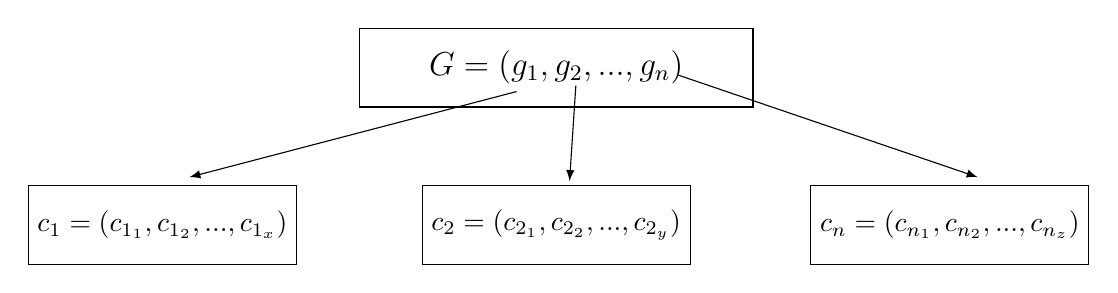
\begin{tikzpicture}
% two boxes
\node[draw,minimum width=5cm, minimum height=1cm] (a) at (5,0) {\large $G = (g_{1} ,  g_{2} ,...,  g_{n})$};
\node[draw,minimum width=3cm, minimum height=1cm] (b) at (0,-2) {$c_{1} = (c_{1_1},c_{1_2},...,c_{1_x})$};
\node[draw,minimum width=3cm, minimum height=1cm] (c) at (5,-2) {$c_{2} = (c_{2_1},c_{2_2},...,c_{2_y})$};
\node[draw,minimum width=3cm, minimum height=1cm] (d) at (10,-2) {$c_{n} = (c_{n_1},c_{n_2},...,c_{n_z})$};

\path (a.east) -- (a.south west) coordinate[pos=0.6] (a1);
\path (b.west) -- (b.north) coordinate[pos=1.2] (b1);
\draw[latex-] (b1) -- (a1);

\path (a.east) -- (a.south west) coordinate[pos=0.45] (a2);
\path (c.west) -- (c.north) coordinate[pos=1.1] (b2);
\draw[latex-] (b2) -- (a2);

\path (a.east)  -- (a.south west) coordinate[pos=0.19] (a3);
\path (d.west) -- (d.north) coordinate[pos=1.2] (b3);
\draw[latex-] (b3) -- (a3);
\end{tikzpicture}
 \caption[Symbolic goal, geometric subgoals and constraint lists]
 {G is the symbolic goal which is segmented into geometric subgoals of $g_{1},...,g_{n}. c_{1}...c_{n}$ represents associated list of constraints}
 \label{fig:s}
\end{figure}

\subsubsection{Monitoring}
\begin{figure}[htbp] %  figure placement: here, top, bottom, or page
   \centering
   %\includegraphics[angle=90,width=10cm]{images/tbox.jpg}
   \includegraphics[width=12cm]{images/snp3.pdf}
   \caption{Monitoring component}
   \label{Fig:Data flow summery}
\end{figure}

The purpose of this component is twofold:
  \begin{itemize}
   \item The \textit{Monitoring} component acts as a coordinator between the \textit{Scheduler} and the motion(path) planner.
   \item Monitoring the working of the motion planner while it attempts to reach the given goal/sub goal.
\end{itemize}
The \textit{Monitoring} component queries the \textit{Scheduler} for a subgoal(with constraints) and 
sends it to the motion planner depending on its status(whether the planner is free).
It then monitors the motion(path) planner executing the given subgoal.
The motion planner notifies the \textit{Monitoring} component about the completion of the sub goal by firing an event.
The motion planner triggers a failure event if the previous sub goal is not achieved, notifying the \textit{Monitoring} component about the failure.
In situations of failure the \textit{Monitoring} component informs the \textit{Navigation Failure Diagnosis} unit.\\

Another important function the \textit{Monitoring} component is expected to perform is setting appropriate parameters\footnote[6]{ROS Navigation stack consist of a set of parameters for (global and local) planners which could be set to customize the behavior of the planners. \url{http://wiki.ros.org/navigation/Tutorials/RobotSetup}. [Online]. Accessed: Oct. 22, 2013] } 
for the motion planner to satisfy the given constraints. 
However, this might not be necessary for some constraints.
For instance, in our work the tolerance limit constraint associated with semantic positions has a different role to play.
It is used for the purpose of monitoring and helps in deciding when to conclude that the given subgoal is achieved.
Hence, the constraint of tolerance limit is not set by the \textit{Monitoring} component.

\subsubsection{Navigation Equations}
\label{sec:ne}
\begin{figure}[htbp]
 \centering
 \includegraphics[width=8.5cm]{images/snp4.pdf}
 \caption{Navigation Equation component}
 \label{Fig:Data flow summery}
\end{figure}

As the name suggests, \textit{Navigation Equations} component contains a set of equations(rules) which can perform certain calculations \cite{1,21}.
The calculations are performed on the properties of the \textit{semantic positions}, that is on \textit{Location, Orientation} and \textit{Tolerance}
properties which have symbolic values.
Example: \textit{Tolerance} can have symbolic values such as \textit{soft/medium/hard}.
These symbolic values are fed as input to the \textit{Navigation Equations} component which performs calculations on them
to convert them into appropriate numerical values.
For instance, if semantic position of \textit{kitchen-1} has a symbolic value \textit{center} for \textit{Location}, then 
these values are fed to the \textit{Navigation Equations} component. 
The component returns a numerical value for the symbolic value \textit{center} using the equation mentioned below:\\

\begin{center}
\begin{Large}
$ x_{center} = \frac{ w_{l} + x + w_{r} }{2}$
 
$y_{center} = \frac{ h_{l} + h + h_{r} }{2}$
\end{Large}
\end{center}

 \begin{figure}[htbp]
 \begin{center}
 \includegraphics[width=10cm]{images/geometry.png}
 \caption[Navigation equation example(up). Region geometry(down) represented by triple \cite{8}]
 {Navigation equation example(up). Region geometry(down) represented by triple $G_{R}$=\textit{(x, y, w, h, $\theta$, $w_{l}$, $h_{l}$, $y_{l}$, $w_{r}$, $h_{r}$, $y_{r}$)} \cite{8}} 
\label{Fig:Data flow summery}
\end{center}
\end{figure}

Similar equations exist for other symbolic values of \textit{Location} and for other properties of semantic positions.
These symbolic values and their definitions could be changed depending on the domain. 
Maintaining equations in a separate component helps to reduce the complexity of the system by decreasing the number of facts to be stored explicitly in the map \cite{1}.
\subsubsection{Map cache}
\begin{figure}[htbp]
 \centering
 \includegraphics[width=12cm]{images/snp5.pdf}
 \caption{Map cache component}
 \label{Fig:Data flow summery}
\end{figure}

The \textit{Map cache} temporarily maintains the environment information relevant for the navigation task being executed.
For instance, in our example, the \textit{Map cache} component maintains occupancy grid maps of \textit{livingroom-1, doorway-1, kitchen-1} along with their topological connectivity.
It also maintains their semantic positions.
Other units like the \textit{Semantic Navigation planner} or \textit{Navigation Failure Diagnosis}  query the \textit{Map cache} 
component for environment information. 
For the first time, the \textit{Map cache} queries the \textit{Environment Model} about environment information, after receiving a request about it from the \textit{Navigation planner} component.\\
This information is then maintained by the \textit{Map cache} either until the symbolic goal is achieved or till a new request is generated by the \textit{Navigation planner} component.
If some additional information is required while execution, for instance by the \textit{Navigation Failure Diagnosis} unit while dealing with unexpected situations(failures), 
it is queried to the \textit{Environment model} via the \textit{Map cache} component.

\subsubsection{Localization cache}
\begin{figure}[htbp]
 \centering
 \includegraphics[width=12cm]{images/snp6.pdf}
 \caption{Localization cache component}
 \label{Fig:Data flow summery}
\end{figure}

The \textit{Localization cache} component maintains a constant update of the robot's current location 
(semantic+topological+metric).
It gets its input from the on-line SLAM algorithm.
%Based on this it will calculate the average probability of location.
The \textit{Monitoring} and other components query the\textit{ Localization cache} for the robot's current semantic location.

\subsubsection{Navigation Failure Diagnosis(\textit{Reasoning and Recovery})}
\begin{figure}[htbp]
 \centering
 \includegraphics[width=12cm]{images/snp7.pdf}
 \caption{Navigation Failure Diagnosis Unit}
 \label{Fig:Data flow summery}
\end{figure}
During the execution of the given sub-goal, if there is a failure,
it is notified to the \textit{Navigation Failure Diagnosis} unit by the \textit{Monitoring} component by triggering a failure event.
The \textit{Navigation Failure Diagnosis} unit then takes control over the low level planners\footnote[7]{Low level planners include the global planner at the motion planning level and the local planner at the controller level as shown in Figure~\ref{fig:SysArc}} 
to overcome the situation.
While the \textit{Navigation Failure Diagnosis} unit is trying to overcome the unexpected situation, it notifies the \textit{Monitoring }component to wait until the recovery is done.
If no solution works for recovering from the situation, the high level (task/symbolic) planner is notified about the symbolic goal failure. \\

However, Failure Diagnosis and Reasoning in robotics are vast fields and under active research.
Hence in this work, we consider Failure Diagnosis for navigation at a naive level. The \textit{Navigation Failure Diagnosis} unit 
needs thorough research and evaluation which is out of the scope of this work.
Our \textit{Recovery} component consists of a set of recovery behaviors which are initiated to recover from unexpected situations.
For instance, one of the recover behaviors our \textit{Recovery} component has is the rotate recovery behavior\footnote[8]{The current ROS Navigation Stack has such a rotate recovery behavior. 
Details of this can be found on: \url{http://wiki.ros.org/rotate_recovery}}.\\

\iffalse 
\subsection{Significance of adding semantic positions for \textit{Regions} and \textit{Objects}:}
\begin{itemize}
  \item In this work, to begin with, our semantic positions will be represented by three properties, namely:
  \begin{itemize}
    \item Location of SP: center/east/west/north/south/north-east/north-west/south-east/southth-west
    \item Orientation of SP: east/west/north/south
    \item Tolerance for the SP: soft/medium/hard
  \end{itemize}
  \item The location and orientation properties are concerned with the x-y co-ordinate (location) of the robot and its rotation angle (orientation) at that location.
  \item The tolerance property is of importance here for navigation.
  \item It determines how close the robot is expected to go to the semantic position.
  \item Usually rooms and other categories of region concept will have soft or medium tolerance.
  \item Objects will mostly have hard tolerance.
  \item However, these assumtions may cahnge depending on the application domain.
  \item This property will be helpful for navigation in the following way:
  \item Usually a robot has to go to any room and has to navigate towards some object.
  For example, for a home assistant robot, it has to go to the kitchen and dock a fridge to pick-up a milk bottle, or dock to the dinner table for cleaning it, or dock to a oven and so on.
  \item For all such situations it is acceptable if the robot does not eaxctly reach the kitchen's semantic position since it has to go to other position (semantic position fo the object to be manipulated).
  \item This will help to deal with situations such as if a person or other obstacle is standing on the semantic position of the room.
  \item Also it might save cost, since one the robot is in the room it can start executing its next path plan. \\\\\\\\
      
    
    \item Location: Indicate the location on x-y plane.
    \item However, in this approach we make use of concepts instead of numerical values to indicate the location.
    \item The location concept will have following instances: center, east, west, north, south.
    \item We can have additional/different instances of the concept location depending on the needs of the domain.
    \item Orientation: The orientation concept will have following four instances: north, south, east, west.
    \item Tolerance: The tolerance concept will have three instances: soft, medium an hard.
    \item soft tolerance will usually be assigne to semantic positions belonging to Region instances.
    \item For instance suppose robot is approaching the kitchen,that is to the semantic position(tolerance: soft) of kitchen. 
    \item soft tolerance will indicate the navigation planning system that it is not required for the robot to be exactly(in terms of x,y cordinates and orientation) at the semantic position.
    \item Instead, the navigation system can conclude that the goal(sub-goal) is achieved as soon as its localization unit etects that the robot has reached the kitchen.
    \item We believe this will help the navigation system to be flexible and help to deal with unexpected situations. Details of the same areexplained in next section.
    \item The locationa dn orientation concepts are adopted from the approach in \cite{8}.
    \item However, adding tolerances to the semantic positions is the contribution of this work.
  
\end{itemize}
\fi